% @Author: Macsnow
% @Date:   2017-05-24 17:04:21
% @Last Modified by:   Macsnow
% @Last Modified time: 2017-05-30 03:12:12

\section{Addtional Problems}

\begin{enumerate}
    \item Explain precisely following abbreviations:
    \begin{itemize}
        \item[-] AS, RIP, OSPF, IGMP, EIGRP, ICMP, BGP, ARP, RARP, CIDR, DHCP, MTU
    \end{itemize}

    \textbf{Answer:}

    \begin{itemize}
        \item AS

        Within the Internet, an autonomous system (AS) is a collection of connected Internet Protocol (IP) routing prefixes under the control of one or more network operators on behalf of a single administrative entity or domain that presents a common, clearly defined routing policy to the Internet.

        \item RIP

        The Routing Information Protocol (RIP) is one of the oldest \textbf{distance-vector} routing protocols which employ the hop count as a routing metric. RIP prevents routing loops by implementing a limit on the number of hops allowed in a path from source to destination.

        \item OSPF

        Open Shortest Path First (OSPF) is a routing protocol for Internet Protocol (IP) networks. It uses a \textbf{link state routing (LSR)} algorithm and falls into the group of interior gateway protocols (IGPs), operating within a single autonomous system (AS).

        \item IGMP

        The Internet Group Management Protocol (IGMP) is a communications protocol used by hosts and adjacent routers on IPv4 networks to establish multicast group memberships.

        \item EIGRP

        Enhanced Interior Gateway Routing Protocol (EIGRP) is an advanced distance-vector routing protocol that is used on a computer network for automating routing decisions and configuration. The protocol was designed by Cisco Systems as a proprietary protocol, available only on Cisco routers.

        \item ICMP

        The Internet Control Message Protocol (ICMP) is a supporting protocol in the Internet protocol suite. It is used by network devices, including routers, to send error messages and operational information indicating.

        \item BGP

        Border Gateway Protocol (BGP) is a standardized exterior gateway protocol designed to exchange routing and reachability information among autonomous systems (AS) on the Internet.

        \item ARP

        The Address Resolution Protocol (ARP) is a communications protocol used for resolution of Internet layer addresses into link layer addresses, a critical function in the Internet protocol suite.

        \item RARP

        The Reverse Address Resolution Protocol (RARP) is an obsolete computer networking protocol used by a client computer to request its Internet Protocol  (IPv4) address from a computer network, when all it has available is its link layer or hardware address, such as a MAC address.

        \item CIDR

        Classless Inter-Domain Routing (CIDR) is a method for allocating IP addresses and IP routing.

        \item DHCP

        The Dynamic Host Configuration Protocol (DHCP) is a standardized network protocol used on Internet Protocol (IP) networks.

        \item MTU

        In computer networking, the maximum transmission unit (MTU) is the size of the largest network layer protocol data unit that can be communicated in a single network transaction.        
    \end{itemize}

    \item Can ATM network provides QoS support? Why?

    \textbf{Answer:}
    
    Yes, ATM can provide several kind of services, in which CBR(Constant Bit Rate) service model guaranteed lost or delivered late ratio will be less than specified values. This is a kind of QoS support.

    \item Which protocols dose ip layer include?

    \textbf{Answer:}

    \begin{itemize}
        \item IPv4 - Internet Protocol version 4
        \item IPv6 - Internet Protocol version 6
        \item ARP - Address Resolution Protocol
        \item ICMP - Internet Control Message Protocol
        \item IGMP - Internet Group Management Protocol
        \item OSPF - Open Shortest Path First
    \end{itemize}    

    \item Which features has IPv6 packet?

    \textbf{Answer:}

    \begin{itemize}
        \item Expanded addressing capabilities.
        \item A streamlined 40-byte header.
        \item Flow labeling and priority.
    \end{itemize}
\end{enumerate}

\section{Problems on Book}

\begin{enumerate}
    \item[P10.] Consider a datagram network using 32-bit host addresses. Suppose a router has four links, numbered 0 through 3, and packets are to be forwarded to the link interfaces as follows:
    \begin{table}[H]
        \centering
        \begin{tabular}{cc}
            \textbf{Destination Address Range} & \textbf{Link Interface} \\
            11100000 00000000 00000000 00000000 & \\
            through & 0 \\
            11100000 00111111 11111111 11111111 & \\
             & \\
            11100000 01000000 00000000 00000000 & \\
            trough & 1 \\
            11100000 01000000 11111111 11111111 & \\
             & \\
            11100000 01000001 00000000 00000000 & \\
            through & 2 \\
            11100001 01111111 11111111 11111111 & \\
             & \\
            otherwise & 3 \\
        \end{tabular}
        \label{tab:p10}
    \end{table}
    \begin{enumerate}
        \item Provide a forwarding table that has five entries, uses longest prefix matching, and forwards packets to the correct link interfaces.
        \item Describe how your forwarding table determines the appropriate link interface for datagrams with destination addresses:
    \end{enumerate}

    \begin{table}[H]
        \centering
        \begin{tabular}{cccc}
            11001000 & 10010001 & 01010001 & 01010101 \\
            11100001 & 01000000 & 11000011 & 00111100 \\
            11100001 & 10000000 & 00010001 & 01110111 \\
        \end{tabular}
        \label{tab:p10_b2}
    \end{table}

    \textbf{Answer:}

    \begin{enumerate}
        \item longest prefix matching forwarding table shows below:
        \begin{table}[H]
            \centering
            \begin{tabular}{cc}
            \textbf{Prefix Match} & \textbf{Link Interface} \\
            11100000 00 & 0 \\
            11100000 01000000 & 1 \\
            11100000 01000001 & 2 \\
            11100000 01 & 2 \\
            11100001 01 & 2 \\
            otherwise & 3 \\
            \end{tabular}
            \label{tab:forwarding_table}
        \end{table}

        \item Discuss IPs above separately.
        \begin{itemize}
            \item This doesn't match any prefix of the fowarding table, so it is an otherwise situation, foward it through interface 3.
            \item Matched to 11100001 01, therefore foward through interface 1.
            \item Doesn't match any prefix, foward through interface 3.
        \end{itemize} 
    \end{enumerate}

    \item[p22.] Suppose you are interested in detecting the number of hosts behind a NAT. You observe that the IP layer stamps an identification number sequentially on each IP packet. The identification number of the first IP packet generated by a host is a random number, and the identification numbers of the subsequent IP packets are sequentially assigned. Assume all IP packets generated by hosts behind the NAT are sent to the outside world.
    \begin{enumerate}
        \item Based on this observation, and assuming you can sniff all packets sent by the NAT to the outside, can you outline a simple technique that detects the number of unique hosts behind a NAT? Justify your answer.
        \item If the identification numbers are not sequentially assigned but randomly assigned, would your technique work? Justify your answer.
    \end{enumerate}

    \textbf{Answer:}

    \begin{enumerate}
        \item Since each host behind NAT has a \textbf{unique} indentification number and all IP packets are sent outside, we can use a sniffer to record all IP packet and group sequentially packets and specify one host. Then the number of groups are the number of hosts.
        \item No, if identification nubmers are not sequentially assigned, then the technique above can't work because it can't group packets now.
    \end{enumerate}

    \item[P25.] Repeat Problem P24 for paths from x to z, z to u, and z to w.

    \begin{figure}[H]
        \centering
        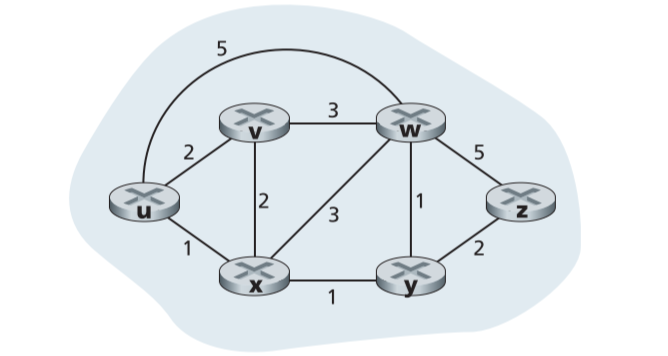
\includegraphics[width=0.8\textwidth]{4th/4-27.png}
        \caption{Figure 4.27}
        \label{fig:4_27}
    \end{figure}

    \textbf{Answer:}

    use tuple to represent paths.

    \begin{itemize}
        \item x to z:
        \begin{enumerate}
            \item (x, y, z)
            \item (x, y, w, z)
            \item (x, w, z)
            \item (x, w, y, z)
            \item (x, v, w, z)
            \item (x, v, w, y, z)
            \item (x, u, w, z)
            \item (x, u, w, y, z)
            \item (x, u, v, w, z)
            \item (x, u, v, w, y, z)
        \end{enumerate}
        \item z to u:
        \begin{enumerate}
            \item (z, w, u)
            \item (z, w, v, u)
            \item (z, w, v, x, u)
            \item (z, w, x, u)
            \item (z, w, x, v, u)
            \item (z, w, y, x, u)
            \item (z, w, y, x, v, u)
            \item (z, y, x, u)
            \item (z, y, x, v, u)
            \item (z, y, x, w, u)
            \item (z, y, x, w, v, u)
            \item (z, y, w, u)
            \item (z, y, w, v, u)
            \item (z, y, w, v, x, u)
            \item (z, y, w, x, u)
            \item (z, y, w, x, v, u)
        \end{enumerate}
        \item z to w:
        \begin{enumerate}
            \item (z, w)
            \item (z, y, w)
            \item (z, y, x, w)
            \item (z, y, x, v, w)
            \item (z, y, x, v, u, w)
            \item (z, y, x, u, v, w)
        \end{enumerate}
    \end{itemize}

    \item[P31.] Consider the three-node topology shown in Figure 4.30. Rather than having the link costs shown in Figure 4.30, the link costs are c(x,y) = 3, c(y,z) = 6, c(z,x) = 4. Compute the distance tables after the initialization step and after each iteration of a synchronous version of the distance-vector algorithm (as we did in our earlier discussion of Figure 4.30).

    \begin{figure}[H]
        \centering
        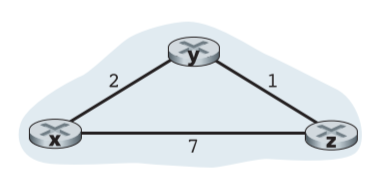
\includegraphics[width=0.8\textwidth]{4th/4-30.png}
        \caption{Figure 4.30}
        \label{fig:4_30}
    \end{figure}

    \textbf{Answer:}

    \begin{itemize}
        \item table of node x
        \begin{table}[H]
            \centering
            \subtable{
                \begin{tabular}{c|ccc}
                     & x & y & z \\
                    \hline
                    x & 0 & 3 & 4 \\
                    y & $\infty$ & $\infty$ & $\infty$ \\
                    z & $\infty$ & $\infty$ & $\infty$ \\
                \end{tabular}
                \label{tab:nodex1}
            }
            \qquad
            \subtable{
                \begin{tabular}{c|ccc}
                     & x & y & z \\
                    \hline
                    x & 0 & 3 & 4 \\
                    y & 3 & 0 & 6 \\
                    z & 4 & 6 & 0 \\
                \end{tabular}
                \label{tab:nodex2}
            }
        \end{table}

        \item table of node y
        \begin{table}[H]
            \centering
            \subtable{
                \begin{tabular}{c|ccc}
                     & x & y & z \\
                    \hline
                    x & $\infty$ & $\infty$ & $\infty$ \\
                    y & 3 & 0 & 6 \\
                    z & $\infty$ & $\infty$ & $\infty$ \\
                \end{tabular}
                \label{tab:nodey1}
            }
            \qquad
            \subtable{
                \begin{tabular}{c|ccc}
                     & x & y & z \\
                    \hline
                    x & 0 & 3 & 4 \\
                    y & 3 & 0 & 6 \\
                    z & 4 & 6 & 0 \\
                \end{tabular}
                \label{tab:nodey2}
            }
        \end{table}

        \item table of node z
        \begin{table}[H]
            \centering
            \subtable{
                \begin{tabular}{c|ccc}
                     & x & y & z \\
                    \hline
                    x & $\infty$ & $\infty$ & $\infty$ \\
                    y & $\infty$ & $\infty$ & $\infty$ \\
                    z & 4 & 6 & 0 \\
                \end{tabular}
                \label{tab:nodez1}
            }
            \qquad
            \subtable{
                \begin{tabular}{c|ccc}
                     & x & y & z \\
                    \hline
                    x & 0 & 3 & 4 \\
                    y & 3 & 0 & 6 \\
                    z & 4 & 6 & 0 \\
                \end{tabular}
                \label{tab:nodez2}
            }
        \end{table}
    \end{itemize}

    \item[P35.] Describe how loops in paths can be detected in BGP.

    \textbf{Answer:}

    since AS-PATH is visible to a source AS, then the loop detection is to check if its own ASN in the AS-PATH.
\end{enumerate}

